\chapter{Arquitectura}
\label{chap:architecture}

%Your text goes here!

%\todoany{Explain the final software development process used by your team. Explain each of your decisions and how it evolved over time, e.g., show how your kanban looks like, how you conducted your retrospectives, the main action points from the retrospectives and how much you were able to apply them, how software quality is part of your process, etc. In addition, discuss the main points that emerged in your retrospective meetings, and what you, as a team, have changed in your process throughout the time. An example of how this can look is provided below (replace it with your own and write one for every retrospective you do). Please remember also in this chapter: less is more!}

\section{Introduction}

En esta sección se mostrará la arquitectura del asistente virtual web. Para facilitar la comprensión de la arquitectura empleada, se dispone de un esquema detallado del sistema expuesto en la figura 2.1. En ella se muestran los distintos agentes participantes en el sistema, así como las infraestructuras principales y sus relaciones.



\begin{figure}[h]
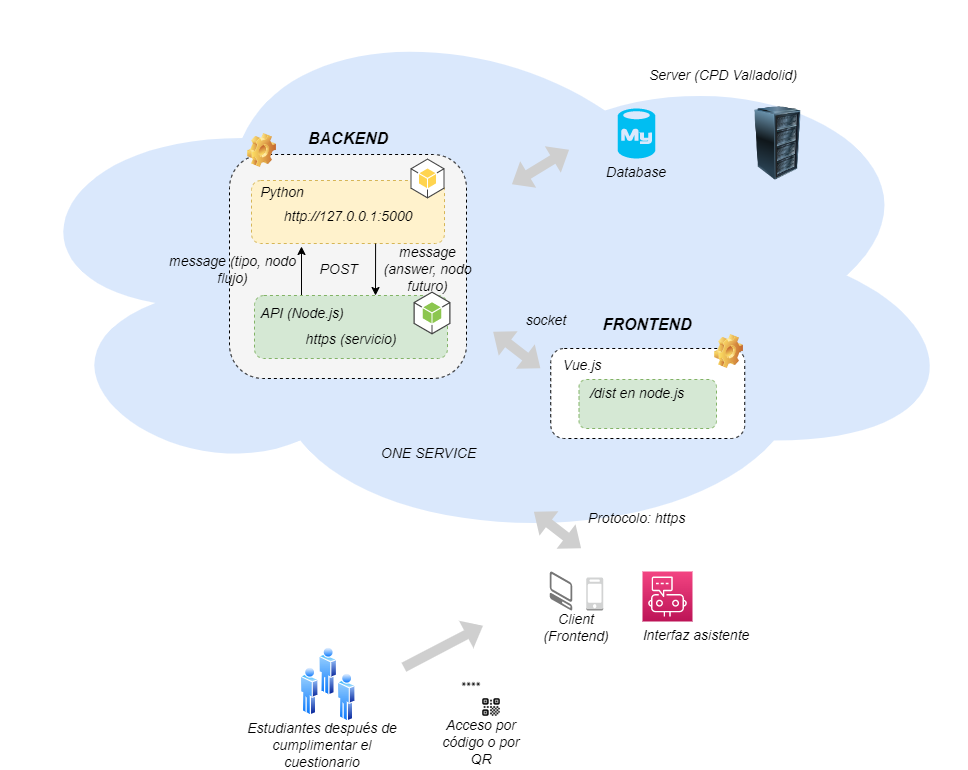
\includegraphics[width=\textwidth]{figures/ArquitecturaDPS.png}
\caption{Arquitectura actual del sistema}
\label{fig:architecture}
\end{figure}




La arquitectura del sistema es una parte fundamental de cualquier desarrolla y permite el correcto diseño. Una arquitectura segura debe ser robusta frente ataques y debe comprender siguientes criterios \cite{ule}: 

\begin{itemize}
    \item Disponibilidad: se denomina disponibilidad a la disposición de los servicios a ser usados cuando sea necesario. La carencia de esta disponibilidad supone una interrupción del serivico y puede afectar directamente a la productivdad de las organizaciones. El asistente virtual funciona bajo demanda con un objetivo simple: recoger una opinión más detallada de los usuarios. Los usuarios suelen ser propensos a no proporcionar opiniones por su propia voluntad, a no ser que un agente externo les incite a participar. La disponibilidad de este servicio es clave en la recolección de estas opiniones, dado que su interrupción o mal funcionamiento puede derivar en una mala experiencia o desuso del asistente.
    \item Integridad: se corresponde con el mantenimiento de las características de completitud y corrección de los datos. Los mensajes enviados entre el asistente y los usuarios debe evitar ser manipulado por terceros, con el fin de evitar la manipulación de las opiniones.
    \item Confidencialidad: la información debe únicamente llegar a las personas autorizadas. Contra la confidencialidad o secreto pueden darse fugas y filtraciones de información, así como accesos no autorizados. En este caso el sistema no trabaja con datos personales de usuarios, no obstante la filtración de las opiniones de los usuarios, así como el acceso a usuarios no autorizados (usuarios que no accedieron al curso previamente) puede derivar en toma de datos que distorsionen la veracidad de las opiniones.
    \item Autenticidad: Propiedad o característica consistente en que una entidad es quien dice ser o bien que garantiza la fuente de la que proceden los datos. Se requiere mantener la autenticidad de los datos y la autenticidad de los usuarios, evitando suplantación de identidad.
    \item Trazabilidad: Aseguramiento de que en todo momento se podrá determinar quién hizo quué y en qué momento. El asistente virtual lleva un registro de información de todas las comunicaciones con el id del usuario.
\end{itemize}
 

\section{Estado actual}

En esta sección se pretende definir el estado actual del sistema. 


\begin{itemize}
    \item Alojamiento: El sistema se encuentra alojado en un servidor físico del CPD del Parque Científico de la Universidad de Valladolid que cuenta con la ISO27001 \cite{ISO27001}. Dispone de configuración de firewall para protección de los servicios alojados. Características del servidor:
\begin{itemize}
        \item El sistema tiene un ancho de banda asegurado a internet Full Dúplex: 2 Mb.
        \item Tiempo de respuesta en días laborales: 20 minutos.
        \item Tiempo de resolución de incidencias críticas en días laborales: 40 minutos.
        \item Tiempo de respuesta en días no laborales y festivos: 1 hora.
        \item Tiempo de resolución de incidencias críticas en días no laborales y festivos: 2 horas.
        \item Disponibilidad del servicio de alojamiento superior al 95\% (salvo causas de fuerza mayor por intervenciones de mantenimiento y pruebas).
\end{itemize}
    \item Relación arquitectura de los componentes y arquitectura física: El asistente virtual es un web service HTTPS que se encuentra desplegado en una máquina virtual del CPD. El servicio cuenta con un proxy inverso para habilitar el cifrado SSL, instalado y configurado, y se puede acceder a partir del DNS del servicio (evitando errores de SSL). Para desplegar el servicio backend (API) de nodejs se utitliza el administrador de procesos PM2. El microservicio de Python se despliega mediante Flask, framework escrito en Python que permite crear aplicaciones web, en local, dentro de la propia máquina. Además, cuenta con la instalación de un WAF (Web Application Firewall) que añade una capa de seguridad, supervisando, filtrando y/o bloqueando el tráfico HTTP hacia y desde una aplciación web.
    \item Base de datos: El servicio cuenta con una base de datos MySQL Server 8.0 \cite{mysql}, instalada dentro del mismo CPD en una máquina virtual aparte. La administración de esta base de datos es dada por únicamente la cuenta administrador (equipo de soporte del CPD). La base de datos no contiene datos personales de los usuarios que establecen comunicación con el asistente virtual. Las conversaciones se asocian a un id, que es el código de acceso proporcionado a los usuarios de forma manual en el centro. Los códigos, a su vez, están relacionados con los formularios cumplimentados con las opiniones del curso.
    \item Servicios: El backend del sistema (API) se encuentra desarrollado en Node.js mediante el framework Express y el frontend está desarrollado en Vue.js. El sistema cuenta con un servicio web service y el frontend de la aplicación (interfaz del chatbot) se integra dentro del backend mediante la carpeta /dist (carpeta que contiene la versión minimizada del código fuente y se utiliza en las aplicaciones en producción). El servicio que trata la lógica del asistente virtual está desarrollado en Python y se despliega en local dentro de la máquina virtual del propio servidor. A través del puerto 443, se expone el servicio del asistente virtual a Internet (se utiliza DNS). El servidor de aplicaciones y la base de datos se encuentran en máquinas distintas suponiendo una gran ventaja desde un punto de vista de seguridad. No hay desventajas por latencia en las comunicaciones.
\end{itemize}




\section{Problemas encontrados}

A raiz del estudio de la arquitectura y del desarrollo del proyecto se han detectado posibles problemas que han de ser solucionados:

\begin{itemize}
    \item El acceso a la aplicación no tiene un sistema de autenticación. Cualquier usuario podría acceder al asistente virtual si tuviera la dirección web. Aunque el asistente virtual para entablar comunicación con los usuarios en un primer lugar pide al usuario que introduza el código que les ha proporcionado el centro de forma manual, no hay ningún trato de intentos de introducción de código. Además el código es un código numérico de 6 dígitos, lo que podría presentar un problema de seguridad por ataques o suplantación de la identidad de los usuarios.
    \item El código de acceso es de un único uso, pero tiene duración ilimitada.
    \item Guías de estilo. Durante el desarrollo no se han seguido las guías de estilo en ninguno de los lenguajes utilizados (JavaScript y Python). En el desarrollo han intervenido tres desarrolladores (un desarrollador Frontend, un desarrollador Backend y un desarrollador backend Python).
    \item Archivos de logs: Hay logs del servicio pm2 en el servidor; no obstante si sucede un error durante la ejecución, no queda registrado.
    \item Tiempo de incidencias: A pesar de que el CPD ofrece un tiempo de respuesta todos los días del año, el equipo de desarrollo no ha definido ningún plan ante incidencias por parte del cliente. Por otra parte, el tiempo de respuesta ante las incidencias los fines de semana son altos dado que los cursos suelen finalizar entre el sábado y domingo y son esos días de la semana con más tráfico hacia el asistente.
    \item Control: Las conversaciones quedan registradas en la base de datos, pero no hay un control de acceso a la web de modo que no se conoce cuánto tráfico externo acceder a la web sin que haya establecido una comunicación con el asistente.
\end{itemize}


\section{Soluciones propuestas}

En esta sección se proponen las siguientes soluciones a los problemas encontrados:

\begin{itemize}
    \item Acceso a la aplicación: Debido a que el sistema, como requisito del cliente, no recoge información personal de los usuarios, no se pueden autenticar por vía clásica (email o username y contraseña). Además, este sistema debe ser ligero y optimizar UX/UI de los usuarios para que no resulte pesado interactuar con el asistente. Es por ello por lo que se puede incidir en el código proporcionado, modificando su estructura y creando un código compuesto por las directrices que propone OWASP, \cite{owasp}, para el tratamiento de contraseñas de usuario.
    \item El código de acceso debe tener un periodo de caducidad. El periodo de caducidad propuesto debe ser hasta el tratamiento de los datos de las encuestas, que coincide con 1 mes antes del inicio de cada curso (los cursos se realizan dos veces por año). El centro tiene su disposición el contacto de los alumnos, por lo que podría envias un correo electrónico general recordando hacer uso del asistente previo a la caducidad del código.
    \item Guías de estilo. Se deberían utilizar guías de estilo de cada propio lenguaje de programación. Cada framework utilizado tiene su propia guía de estilos: Node.js \cite{nodejsstyleguide}, Vue.js \cite{vuejsstyleguide} y Python \cite{pythonstyleguide:2001}.
    \item Archivos de logs: Se deberían incluir más puntos de recogida de logs dentro del código desarrollado del asistente para tener mayor precisión en el tratamiento de errores.
    \item Tiempo de incidencia: El equipo debe elaborar un plan de respuesta a incidencias. 
    \item Control: En el estado actual, el sistema crea una nueva conversación en la base de datos cuando el usuario hace click en el plugin de la web e introduce su código de usuario. Se pierde mucho control del tráfico que puede existir en la web, por lo que se propone modificar la estructura de desarrollo y que se active el plugin del asistente cuando un usuario acceda a la web. Dado que es una web específica para el asistente virtual no tiene desventaja sobre UX/UI del usuario en la web. De esta manera se puede llevar un control más preciso.
\end{itemize}



 








%\subsection{Example Week}

%\subsubsection{Positive Points}
%\begin{itemize}[noitemsep]
%    \item Nice communication.
    %\item We delivered all the features we promised!
%\end{itemize}

%\subsubsection{Negative Points}
%\begin{itemize}[noitemsep]
    %\item One story was not well estimated. \textbf{Action point:} re-discuss %this story in the next sprint planning.
    %\item We lacked day-to-day communication. \textbf{Action point:} create a %WhatsApp group.
%\end{itemize}
